\documentclass[11pt,a4paper]{article}
\usepackage[margin=2.3cm]{geometry}
\usepackage{amsmath,amssymb}
\usepackage{graphicx}
\usepackage{booktabs}
\usepackage{siunitx}
\usepackage{tikz}
\usepackage{hyperref}
\usepackage[font=small]{caption}
\graphicspath{{figures/}}

\title{Second-order mimetic velocity reconstruction with buildings\\
       in \texttt{palm\_ftle}: first- versus second-order FTLE}
\author{pv\_ftle --- branch \texttt{palm2ndorder}}
\date{\today}

\begin{document}
\maketitle

\begin{abstract}
\texttt{palm\_ftle} now reconstructs the PALM wind with second-order mimetic
elements (\texttt{--order 2}, the new default) in a new double-precision C++
integrator. Each velocity component is quadratic across the cell and linear
along each face, while every face keeps its exact flux. Buildings need special
care, because a second-order reconstruction draws on neighbouring faces: faces
are classified as fluid, wall or solid from PALM's fill values; a wall carries
zero flux and no tangential slope; slopes and curvatures use fluid data only;
and the velocity inside a building is zero. Against exact trajectories of an
analytic divergence-free wind around three buildings, the second-order
reconstruction is 2.5--9 times more accurate than the first-order one near the
buildings and 5--50 times away from them, and no particle ends up inside a
building. On a PALM large-eddy simulation of a built-up area
($\SI{4}{m}$ grid, $T=\SI{-10}{s}$), the two orders give the same FTLE structures
everywhere. The differences are largest in the lowest layer (\SIrange{4}{8}{m}),
where a third of the cells are buildings and the first-order FTLE is biased
low by 9\% of the FTLE scale, and they fall to a median of 2\% above
\SI{30}{m}. The differences are more than 100 times larger than the time-stepping
error, so they come from the reconstruction.
\end{abstract}

\section{Introduction}

\texttt{palm\_ftle} computes the finite-time Lyapunov exponent (FTLE) from
PALM output. Particles are seeded at the corners of a window of the
rectilinear PALM grid, advected over a time $T$ (negative for backward FTLE)
with RK4, and the FTLE is computed in each cell from the gradient of the flow
map. Until now the wind between the faces was reconstructed with the
lowest-order Raviart--Thomas (RT$_0$) element: each component is linear between
its two faces and constant along each face, so the tangential wind jumps from
one cell to the next. \texttt{wrf\_ftle} already offers a second-order element.
This report describes how it was carried over to PALM, where the main new
difficulty is buildings, and compares the FTLE computed with the two orders.

\section{Second-order reconstruction}

PALM stores the velocity normal to each face of an Arakawa C grid: $u$ on the
$x$ faces, $v$ on the $y$ faces and $w$ on the $z$ faces. Let $(\xi,\eta,\zeta)\in[0,1]^3$
be the local coordinates of a point in cell $(i,j,k)$, and consider $u$ (the
other components are analogous). With $u_0$ and $u_1$ the values on the west and
east faces, the first-order reconstruction is
\begin{equation}
  u^{(1)} = (1-\xi)\,u_0 + \xi\,u_1 .
\end{equation}
The second-order ($Q_{2,1,1}$) reconstruction adds a linear variation along each
face and a quadratic term across the cell:
\begin{equation}
  u^{(2)} = (1-\xi)\,\tilde u_0 + \xi\,\tilde u_1 + \tfrac12\,c\,\xi(\xi-1),
  \qquad
  \tilde u_f = u_f + s^\eta_f\,(\eta-\tfrac12) + s^\zeta_f\,(\zeta-\tfrac12).
  \label{eq:order2}
\end{equation}
\begin{itemize}
  \item The tangential slopes $s^\eta_f$, $s^\zeta_f$ of face $f$ are the central
        differences $\tfrac12(u_{f+1}-u_{f-1})$ of the neighbouring faces in
        the $y$ and $z$ directions.
  \item The curvature $c$ is the second difference $u_{-1}-2u_0+u_1$ (or
        $u_0-2u_1+u_2$) along $x$, averaged over the two faces of the cell.
\end{itemize}
The slope terms have zero mean over each face, and $\xi(\xi-1)$ vanishes on both
faces, so every face keeps its exact flux and the reconstruction stays
mimetic. The quadratic term lets $\partial u/\partial x$ vary across the
cell, which the first-order element cannot do. On a uniform grid the
reconstruction is exact for any linear wind and is continuous across faces.
The slopes are index-space differences, so on PALM's stretched upper layers
(\SI{4}{m} below \SI{56}{m}, \SI{8}{m} above) the reconstruction is no longer exact for
a linear wind, but it remains much more accurate than the first-order one
(unit test \texttt{test\_order2\_much\_more\_accurate\_on\_stretched\_layers}).

\section{Buildings}

The second-order terms use the faces adjacent to the cell's own faces, so next
to a building they would draw on values inside it. PALM writes the fill value
$-9999$ on every face that touches a building; with \texttt{--zero-fill} (the
default) these become 0. Using such faces as data would treat the inside of a
building as still air, giving spurious tangential slopes along walls. The
second-order reconstruction therefore follows the rules below.

\paragraph{Building mask.} A cell is solid when all six of its faces are
masked. The fill mask is constant in time; for the file used here, a face is
masked exactly when one of its two cells is solid, so the face masks and the
cell mask carry the same information. The ground face that \texttt{palm\_ftle}
adds below \texttt{zw\_xy} is never masked, so a solid cell in the lowest layer
is recognised from its other five faces.

\paragraph{Face types.} Each face is
\begin{itemize}
  \item \emph{fluid} if neither of its cells is solid;
  \item a \emph{wall} if exactly one of its cells is solid --- the normal velocity
        on it is exactly 0;
  \item \emph{solid} if both of its cells are solid.
\end{itemize}

\paragraph{Rules (order 2).}
\begin{enumerate}
  \item A wall face carries zero flux and no tangential slope: the wind
        normal to a wall is zero over the whole wall, including next to
        edges and corners.
  \item The slopes of a fluid face use the neighbouring faces that are not
        solid. A wall's 0 counts as data. The difference is central when both
        neighbours are usable, one-sided when only one is, and 0 when neither
        is.
  \item The curvature uses second differences at fluid faces only, again with a
        wall's 0 counted as data; there is no curvature from a wall face.
  \item The velocity inside a solid cell is zero.
\end{enumerate}
No no-slip condition is imposed: the tangential wind next to a wall comes from
the fluid data, as in the LES, where the wind is resolved only down to the
first grid point off the wall. A component parallel to a wall, such as the
vertical wind in the first fluid cell beside a building, is reconstructed
exactly as in open air, because its faces are fluid faces. Figure~\ref{fig:faces}
shows the classification on a vertical section.

\begin{figure}[ht]
\centering
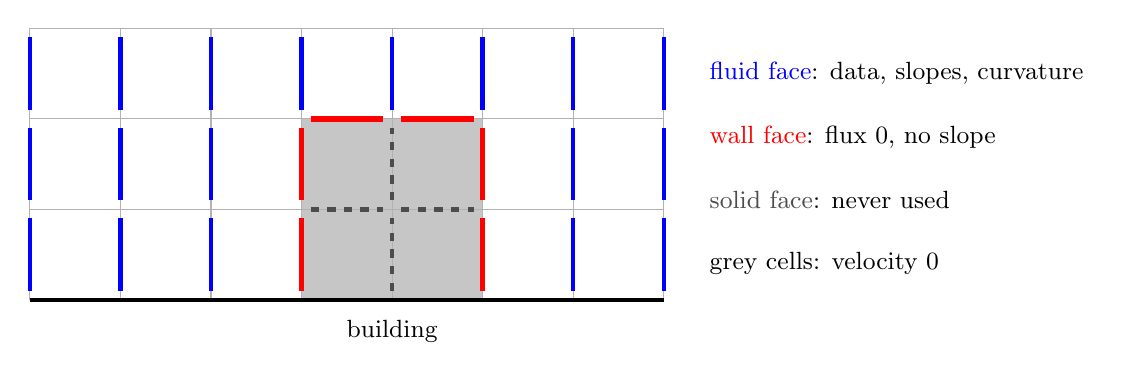
\begin{tikzpicture}[scale=1.15]
  \fill[gray!45] (3,0) rectangle (5,2);
  \draw[gray!60] (0,0) grid (7,3);
  \draw[very thick] (0,0) -- (7,0);
  \foreach \x in {0,1,2,5,6,7} \foreach \y in {0.5,1.5,2.5} \draw[blue, line width=1.6pt] (\x,\y-0.4) -- (\x,\y+0.4);
  \foreach \x in {3,4} \draw[blue, line width=1.6pt] (\x,2.1) -- (\x,2.9);
  \foreach \y in {0.5,1.5} \draw[red, line width=2pt] (3,\y-0.4) -- (3,\y+0.4);
  \foreach \y in {0.5,1.5} \draw[red, line width=2pt] (5,\y-0.4) -- (5,\y+0.4);
  \draw[red, line width=2pt] (3.1,2) -- (3.9,2);
  \draw[red, line width=2pt] (4.1,2) -- (4.9,2);
  \foreach \y in {0.5,1.5} \draw[black!70, line width=1.6pt, dashed] (4,\y-0.4) -- (4,\y+0.4);
  \draw[black!70, line width=1.6pt, dashed] (3.1,1) -- (3.9,1);
  \draw[black!70, line width=1.6pt, dashed] (4.1,1) -- (4.9,1);
  \node at (4,-0.35) {\small building};
  \node[anchor=west] at (7.4,2.5) {\small\textcolor{blue}{fluid face}: data, slopes, curvature};
  \node[anchor=west] at (7.4,1.8) {\small\textcolor{red}{wall face}: flux 0, no slope};
  \node[anchor=west] at (7.4,1.1) {\small\textcolor{black!70}{solid face}: never used};
  \node[anchor=west] at (7.4,0.4) {\small grey cells: velocity 0};
\end{tikzpicture}
\caption{Face classification on an $x$--$z$ section through a building two
cells wide and two cells tall (only the $x$ faces of fluid cells and the faces
around the building are drawn). The slope along $z$ of the fluid $x$ face
left of a wall uses its fluid neighbours; the curvature of $u$ in the cell
left of the wall uses the second difference at that cell's west face, in which
the wall's 0 counts as data.}
\label{fig:faces}
\end{figure}

\paragraph{Particles.} A seed lying exactly on a wall (all seeds on building
surfaces, since seeds sit on grid corners) is assigned to the fluid cell on the
other side of the wall, so it moves with the air beside the building instead
of staying put. If an RK4 step ends inside a building, each coordinate whose
crossing alone leads into the building is clamped just short of the wall, so
the particle slides along it; if it is still inside, the step is undone. The
first-order reconstruction uses the same mask, rules 1 and 4 and the same
particle handling; rules 2 and 3 do not apply to it.

\section{Other changes}

\begin{itemize}
  \item \textbf{New integrator.} \texttt{integrate\_rk4\_rectilinear} in
        \texttt{cpp/ftlecpp.cpp} (OpenMP, one fused RK4 loop per particle)
        replaces the old kernel for \texttt{palm\_ftle}. Positions, times
        and axes are in double precision; the face data stay in single
        precision.
  \item \textbf{Time interpolation.} The old kernel assumed evenly spaced output
        times. The PALM file's times are 0.96--\SI{1.07}{s} apart, so after eight
        outputs the old kernel was \SI{0.065}{s} out. The new integrator
        interpolates on the actual time axis. With frozen wind, the old kernel
        and the new first-order integrator agree to \SI{0.2}{mm} (median).
        \texttt{palm\_ftle\_idx} still uses the old kernel.
  \item \textbf{Command line.} \texttt{--order 1|2} (default 2);
        \texttt{--visualise}, \texttt{--level}, \texttt{--cmax} open the same
        interactive level viewer as \texttt{wrf\_ftle}, with buildings in grey.
  \item \textbf{Tests.} \texttt{tests/test\_palm\_reconstruction.py} (11 tests):
        exactness and continuity on a uniform grid, accuracy on stretched
        layers, zero velocity inside buildings, zero normal velocity everywhere
        on walls and roofs, seeds on walls, particles kept out of buildings,
        and recovery of the building mask from PALM-style face masks. CI
        runs the two PALM cases with order 2 and a third with order 1.
\end{itemize}

\section{Analytic benchmark}

The script \texttt{scripts/bench\_palm.py} builds a divergence-free wind around
three box buildings (\SIlist{24;40;16}{m} tall) in a
$\SI{320}{m}\times\SI{320}{m}\times\SI{64}{m}$ domain:
\begin{itemize}
  \item a sheared mean flow at \ang{25} to the grid;
  \item horizontal vortices;
  \item an $x$--$z$ roll ($|w|\lesssim\SI{0.5}{m/s}$).
\end{itemize}
The stream functions are multiplied by a factor that vanishes on the buildings, so
the walls and roofs are streamlines and the air slides along them, as for the
resolved wind next to walls in an LES ($R=\SI{12}{m}$ wall layer).
Face values are exact face means; exact trajectories are integrated with
$\Delta t=\SI{0.01}{s}$. The 5625 seeds, \SI{8}{m} apart, are integrated over
$T=\SI{-20}{s}$ (median displacement \SI{54}{m}) at \SIlist{8;4;2}{m}
resolution. Seeds on or in buildings, where the analytic flow map is
degenerate, are left out. ``Near'' means seeds within \SI{8}{m} and FTLE cells
within \SI{16}{m} of a building.

\begin{table}[ht]
\centering
\begin{tabular}{lccc ccc}
\toprule
 & \multicolumn{3}{c}{order 1} & \multicolumn{3}{c}{order 2}\\
\cmidrule(lr){2-4}\cmidrule(lr){5-7}
grid spacing (m) & 8 & 4 & 2 & 8 & 4 & 2\\
\midrule
position error near, median (m) & 5.2 & 1.4 & 0.43 & 2.1 & 0.28 & 0.047\\
position error near, 95th pct (m) & 36 & 19 & 9.7 & 18 & 4.3 & 1.4\\
position error away, median (m) & 1.0 & 0.33 & 0.12 & 0.13 & 0.016 & 0.0024\\
FTLE error near, median (\%) & 7.4 & 1.8 & 0.57 & 2.9 & 0.42 & 0.081\\
FTLE error away, median (\%) & 1.5 & 0.47 & 0.16 & 0.29 & 0.032 & 0.0047\\
\bottomrule
\end{tabular}
\caption{Analytic benchmark: errors against exact trajectories. FTLE errors
are relative to the FTLE scale (99th percentile of the exact FTLE,
\SI{0.11}{s^{-1}}). No particle ends inside a building with either order.}
\label{tab:bench}
\end{table}

\begin{figure}[ht]
\centering
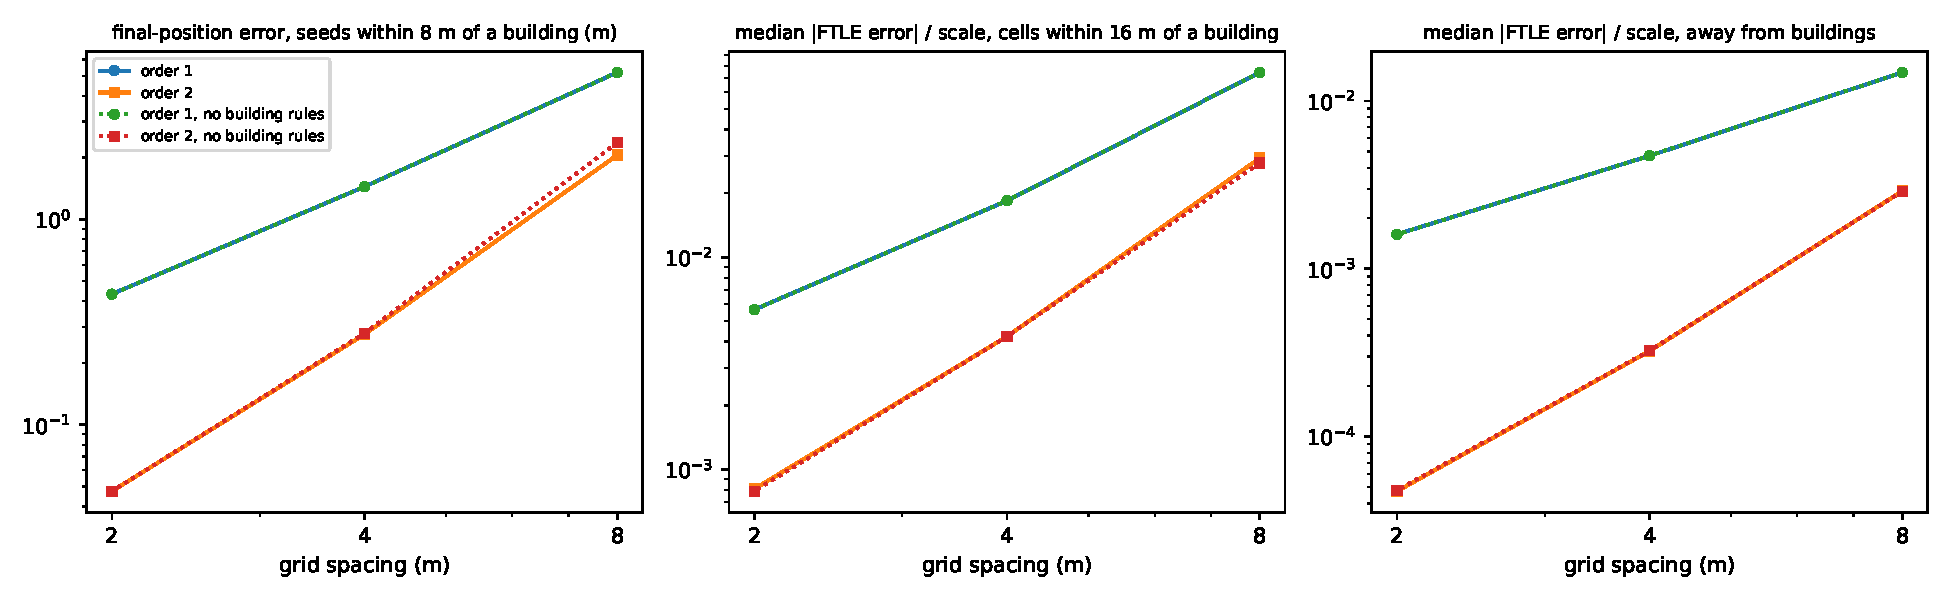
\includegraphics[width=\textwidth]{palm_bench_slip.pdf}
\caption{Analytic benchmark: median errors against grid spacing. Order 1
converges at first order, order 2 at second order. The dotted lines are order 2
without the building rules (all faces used as data, walls included); order 1
is unaffected by them.}
\label{fig:bench}
\end{figure}

Table~\ref{tab:bench} and Figure~\ref{fig:bench} show:
\begin{itemize}
  \item Order 2 converges at second order, order 1 at first order.
  \item Order 2 is 2.5--9 times more accurate near buildings and 5--50 times
        away from them.
  \item The building rules improve the tails at the coarsest grid (95th
        percentile \SI{18}{m} instead of \SI{19}{m}, median \SI{2.1}{m} instead
        of \SI{2.4}{m}). Without them, one particle ends inside a building.
  \item With a no-slip variant of the wind, which vanishes on the walls, the
        rules make almost no difference: the zeros on the walls are then
        accurate data.
\end{itemize}

\section{Comparison on PALM data}

\subsection{Set-up}

The PALM file \texttt{small\_blf\_day\_loc1\_4m\_xy\_N04.003.nc} is a large-eddy
simulation of a built-up area:
\begin{itemize}
  \item horizontal grid spacing \SI{4}{m};
  \item 18 layers, \SI{4}{m} thick up to \SI{56}{m} and \SI{8}{m} above, up to
        \SI{96}{m};
  \item the ground face is reconstructed at \SI{4}{m};
  \item output roughly every second.
\end{itemize}
The FTLE was computed:
\begin{itemize}
  \item in the window $i=20$--100, $j=5$--95 ($\SI{320}{m}\times\SI{360}{m}$,
        $1.4\times10^5$ seeds, 129\,600 cells);
  \item backwards over $T=\SI{-10}{s}$ from time index 20 ($t=\SI{7511}{s}$);
  \item with time-dependent wind;
  \item with 575 RK4 steps (CFL 0.25).
\end{itemize}
In the window, buildings fill 35\% of the lowest layer (\SIrange{4}{8}{m}), 11\%
of the second and 0.6\% of the third; none reaches \SI{16}{m}. Differences are
quoted relative to the FTLE scale $S=\SI{0.24}{s^{-1}}$, the 99th percentile of
the second-order FTLE. The scripts that produce the runs, statistics and
figures are listed in the appendix.

\subsection{Three layers}

Figure~\ref{fig:levels} compares the FTLE at three layers:
\begin{itemize}
  \item the lowest layer (\SIrange{4}{8}{m}), among the buildings;
  \item layer 8 (\SIrange{36}{40}{m}), in the middle;
  \item the top layer (\SIrange{88}{96}{m}).
\end{itemize}

\begin{figure}[p]
\centering
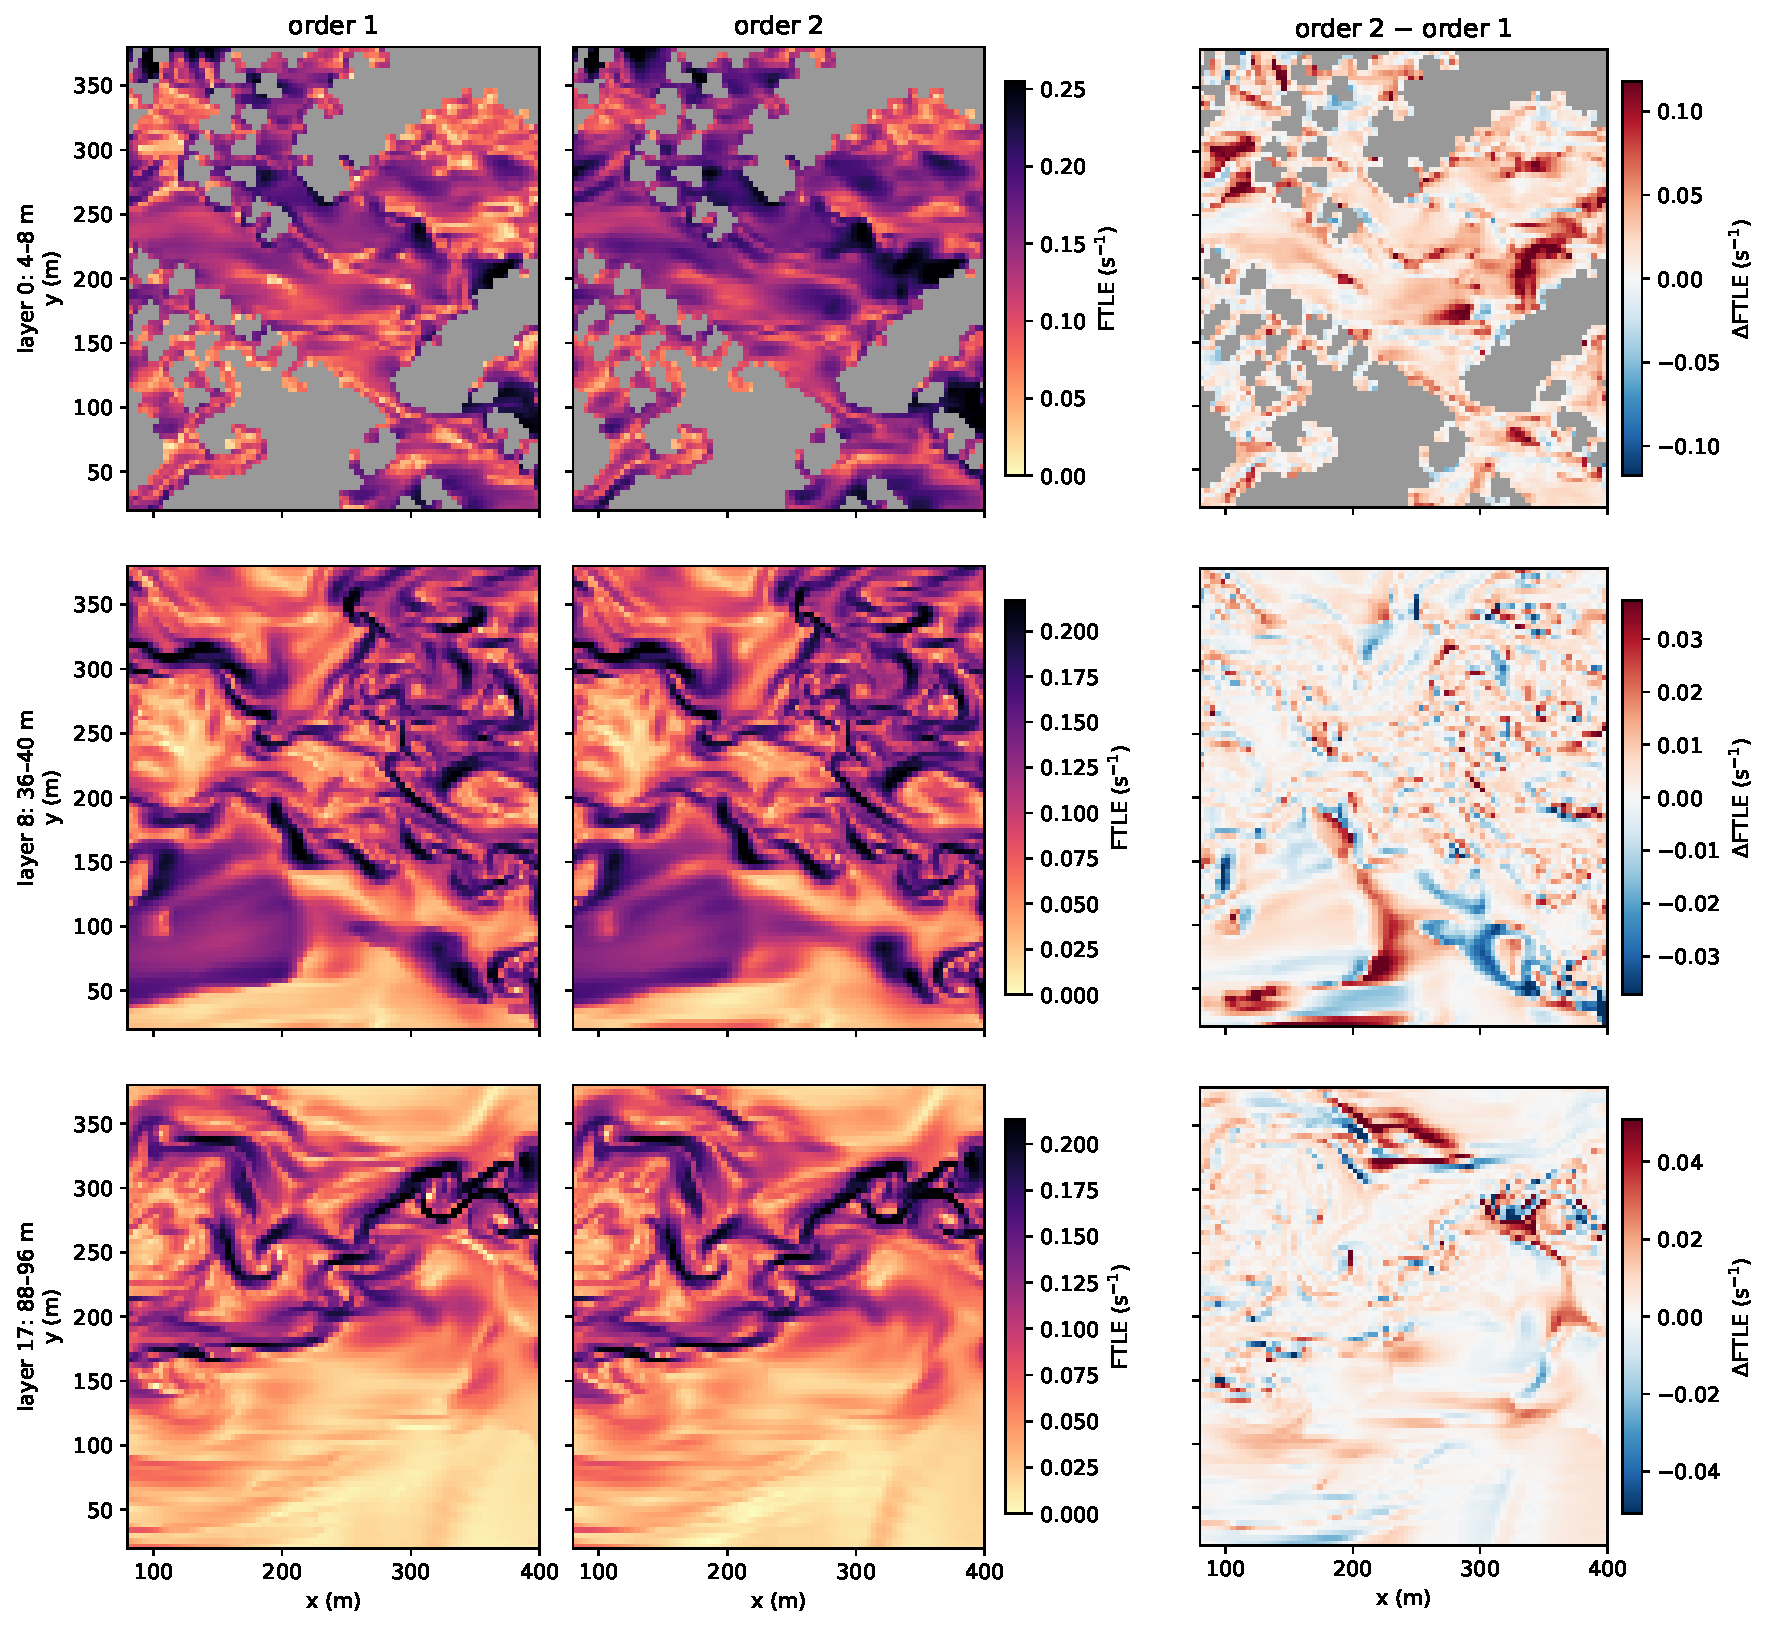
\includegraphics[width=\textwidth]{levels.pdf}
\caption{FTLE ($T=\SI{-10}{s}$) with order 1 (left) and order 2 (centre), and
their difference (right), at the lowest, a middle and the top layer. Buildings
are grey. Each row has its own colour scales; note that the difference scale
of the lowest layer is three times that of the others.}
\label{fig:levels}
\end{figure}

\begin{figure}[ht]
\centering
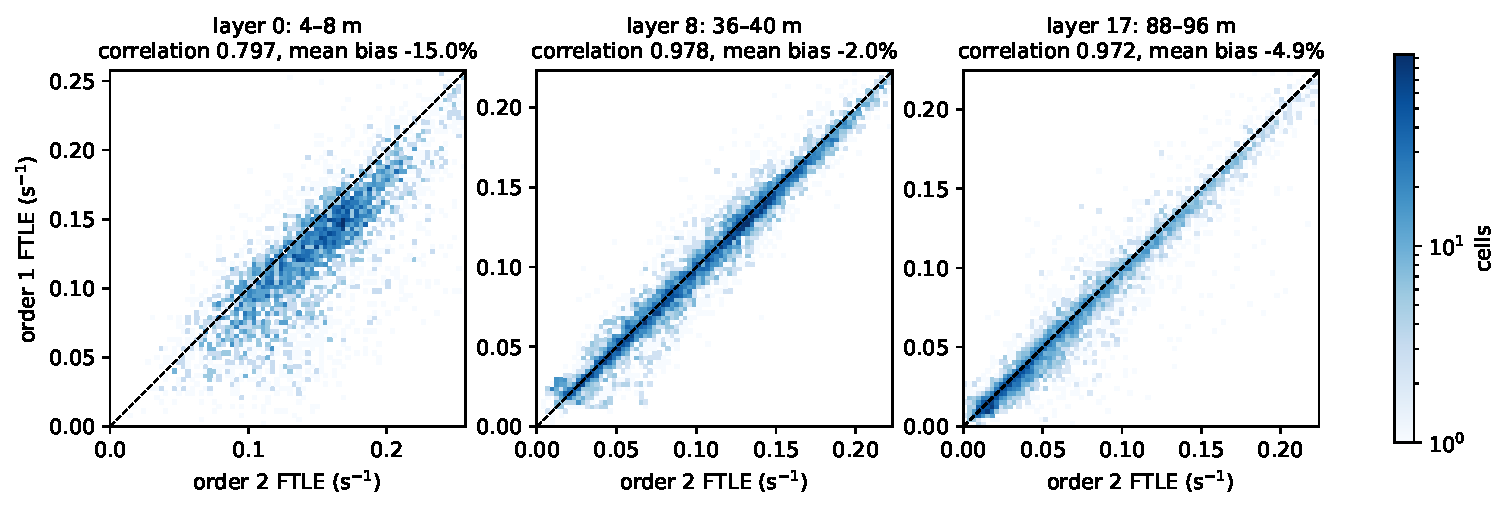
\includegraphics[width=\textwidth]{scatter.pdf}
\caption{Order-1 against order-2 FTLE in every fluid cell of the three layers
(log colour scale). The mean bias is relative to the mean order-2 FTLE of the
layer.}
\label{fig:scatter}
\end{figure}

\paragraph{Lowest layer.} The two orders show the same structures: high FTLE
in the street canyons and in the wakes of building blocks, and low FTLE in the
open area. The differences, however, are large:
\begin{itemize}
  \item median $|\Delta|=8.5\%$ of $S$, 95th percentile 33\%;
  \item correlation 0.80 (Figure~\ref{fig:scatter});
  \item order 1 is lower in most cells, by 9\% of $S$ on average (15\% of
        the layer's mean FTLE).
\end{itemize}
The largest differences are not confined to the cells next to buildings: they
also cover patches of open ground one or more cells away from walls. This is the layer with
the strongest vertical shear. Order 1 holds the horizontal wind constant with
height within each layer, so the shear between the seeds at the bottom and top
of a cell comes only from the jump between layers. Order 2 interpolates
linearly with height, using a one-sided slope at the ground. The low bias
matches the first-order deficit found in the lowest layer of WRF (see the
\texttt{wrf\_ftle} order-2 report).

\paragraph{Middle and top layers.} There are no buildings at these heights and
the agreement is close:
\begin{itemize}
  \item correlation 0.98 and 0.97;
  \item median $|\Delta|$ 2.0\% and 1.8\% of $S$, 95th percentile about 10\%;
  \item bias $-0.9\%$ and $-1.4\%$.
\end{itemize}
The differences sit along the sharp FTLE ridges, where they are signed
(often dipoles), so the ridges shift or sharpen slightly between the two orders but
are not created or removed. At the top the layers are \SI{8}{m} thick, so order 1
is coarser in the vertical and the ridges around $y=\SIrange{280}{340}{m}$ show
the largest differences of that layer.

\subsection{Statistics by layer and distance to buildings}

Figure~\ref{fig:bylevel} shows the median and 95th percentile of the
difference in every layer:
\begin{itemize}
  \item The median decreases steadily from 8.5\% at the ground to 2\%
        at \SI{40}{m}, and stays there.
  \item The bias (order 1 lower) is concentrated in the lowest layer, with
        $-2\%$ in the second and third, and $-1.4\%$ to $+0.1\%$ above.
\end{itemize}
Table~\ref{tab:distance} groups the cells of the whole window by their
distance to the nearest building:
\begin{itemize}
  \item Next to buildings the order difference is three times larger than
        far from them.
  \item The building rules change the order-2 FTLE next to buildings by as
        much as switching from order 1 to order 2 (median 4.5\% vs 5.6\%).
        They make no difference farther than three cells away.
\end{itemize}
Figure~\ref{fig:rules} maps the effect of the rules in the lowest layer: it is
confined to the cells adjacent to walls, and in most of them the FTLE is
higher without the rules.

\begin{figure}[ht]
\centering
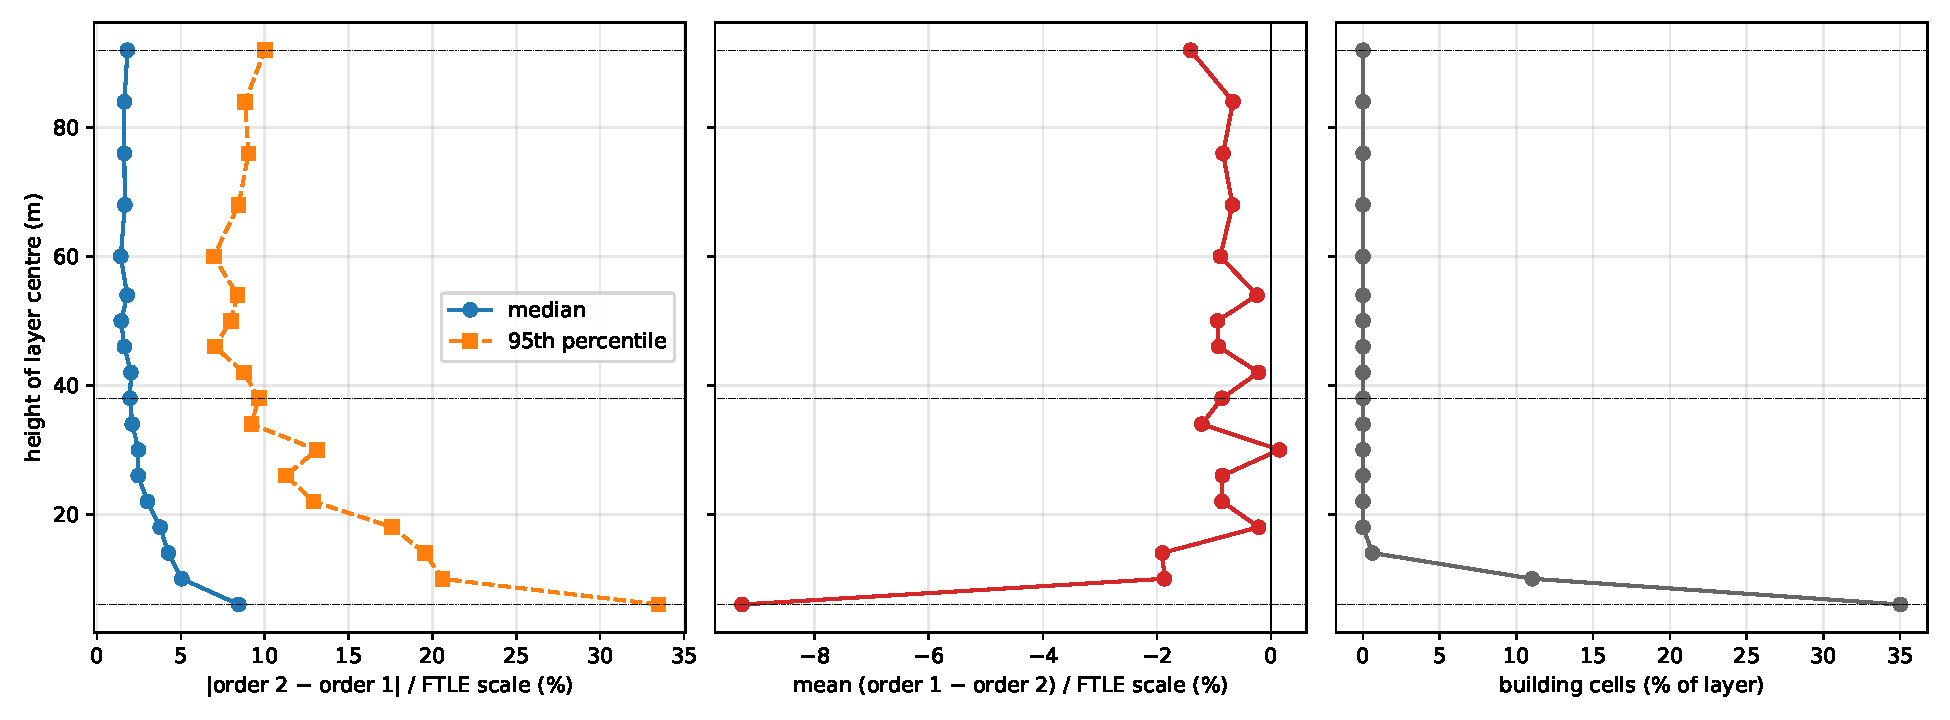
\includegraphics[width=\textwidth]{by_level.pdf}
\caption{By layer: median and 95th percentile of $|$order 2 $-$ order 1$|$
(left), mean order 1 $-$ order 2 (centre), both relative to $S$, and the
fraction of building cells (right). Dotted lines mark the three layers of
Figure~\ref{fig:levels}.}
\label{fig:bylevel}
\end{figure}

\begin{table}[ht]
\centering
\small
\begin{tabular}{lrcccc}
\toprule
distance to building & cells & order 2 vs 1 & rules on vs off & CFL$/4$ (o2) & nudge (o1 / o2)\\
\midrule
1 cell (adjacent) & 6226   & 5.6 / 23 & 4.5 / 21 & 0.03 / 1.9 & 2.4 / 1.8\\
2--3 cells        & 15147  & 4.1 / 19 & 0 / 3.0  & 0.004 / 0.03 & 0.013 / 0.003\\
farther           & 104866 & 2.0 / 11 & 0 / 0    & 0.002 / 0.014 & 0.006 / 0.002\\
\bottomrule
\end{tabular}
\caption{Median / 95th percentile of FTLE differences in \% of $S$, by
chessboard distance to the nearest building cell (in 3D), over all layers.
``CFL$/4$'': four times smaller time step. ``Nudge'': seeds displaced by
\SI{10}{\micro m} at random (median only).}
\label{tab:distance}
\end{table}

\begin{figure}[ht]
\centering
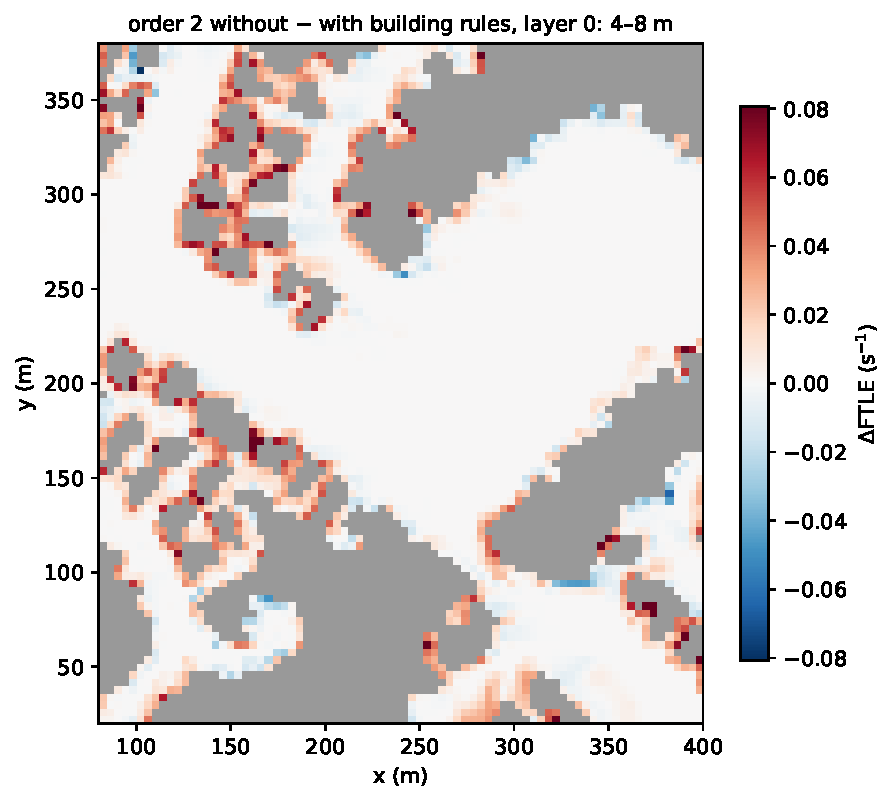
\includegraphics[width=0.6\textwidth]{rules.pdf}
\caption{Effect of the building rules on the order-2 FTLE in the lowest
layer: order 2 with every face used as data (walls and faces inside
buildings) minus order 2 with the rules.}
\label{fig:rules}
\end{figure}

\subsection{Time step and seeds on faces}

The last two columns of Table~\ref{tab:distance} check the numerics:
\begin{itemize}
  \item \textbf{Time step.} Reducing the time step by four changes the
        FTLE by a median 0.002--0.03\% of $S$, 150--1000 times less than the
        difference between the orders, so the comparison measures the
        reconstruction.
  \item \textbf{Seeds on faces, away from buildings.} The seeds lie exactly
        on cell faces, where the first-order tangential wind jumps; nudging
        them by \SI{10}{\micro m} changes the order-1 FTLE three to four times
        more than the order-2 FTLE, whose wind is continuous across fluid
        faces.
  \item \textbf{Seeds on building walls.} Here both orders are sensitive (about
        2\% median): a seed nudged into the building stays there with zero
        velocity, while one nudged out moves with the air. The FTLE of cells
        whose corners lie on walls is ill-defined for either order and should
        be read with care.
\end{itemize}

\section{Conclusions}

\begin{itemize}
  \item The second-order reconstruction in \texttt{palm\_ftle} keeps the exact
        face fluxes, gives a continuous wind across fluid faces, and handles
        buildings by using fluid data only, with zero normal velocity on walls
        and zero velocity inside buildings.
  \item In the analytic benchmark it converges at second order, is 2.5--9 times
        more accurate than order 1 near buildings and 5--50 times away from
        them, and keeps all particles out of buildings.
  \item On PALM data, order 1 and order 2 agree closely above the buildings
        (median difference 2\% of the FTLE scale, correlation 0.97--0.98). In
        the lowest layer they differ by 8.5\% (median), and order 1 is biased
        low by 9\%, consistent with its missing within-layer shear.
  \item Next to buildings the building rules matter as much as the order.
        Without them the second-order wind would be built partly from the
        zeros inside buildings.
  \item Order 2 is the default. Order 1 remains available
        (\texttt{--order 1}) for comparison.
\end{itemize}

\appendix
\section{Reproducing the results}

\begin{verbatim}
python scripts/bench_palm.py OUT FIG --slip      # analytic benchmark
python scripts/palm_order_compare.py small_blf_day_loc1_4m_xy_N04.003.nc CMP
python scripts/palm_order_report_figs.py small_blf_day_loc1_4m_xy_N04.003.nc \
       CMP report/palm_order2/figures
palm_ftle small_blf_day_loc1_4m_xy_N04.003.nc --imin=20 --imax=100 \
       --jmin=5 --jmax=95 --time-index=20 --tintegr=-10 --order=2 --visualise
\end{verbatim}

\end{document}
